\documentclass[11pt,oneside,a4paper]{report}
%for hungarian letters
\usepackage[utf8]{inputenc}

\renewcommand*\thesection{\arabic{section}}
\usepackage{graphicx}
\usepackage{amsmath}
\usepackage{amsfonts}

\usepackage{algorithm}
%for pseudo codes:
\usepackage{algpseudocode}

%for hyperreferences
\usepackage{hyperref}
%--------------------------------------------------------------------------------------
%	Setup hyperref package
%--------------------------------------------------------------------------------------
\hypersetup{
	bookmarks=true,            % show bookmarks bar?
	unicode=false,             % non-Latin characters in Acrobat’s bookmarks
	pdfproducer={Producer},    % producer of the document
	pdfkeywords={keywords},    % list of keywords
	pdfnewwindow=true,         % links in new window
	colorlinks=true,           % false: boxed links; true: colored links
	linkcolor=black,           % color of internal links
	citecolor=black,           % color of links to bibliography
	filecolor=black,           % color of file links
	urlcolor=black             % color of external links
}

%for being able to use more than 10 columns in bmatrix.
\setcounter{MaxMatrixCols}{20}

%setting margin size:
\usepackage{geometry}
\geometry{top=1.5in}
\geometry{margin=1.5in}

\setlength{\parindent}{0pt} % nicer spacing, english style
\setlength{\parskip}{8pt plus 3pt minus 3pt} % nicer spacing, english style

\usepackage{enumitem}	%for being able to set spacing of lists
\setlist{nosep}

\title{Starbucks's Capstone Challenge \\ 
		Report}
\author{Ferenc Török \\ \href{mailto:ferike.trk@gmail.com}{ferike.trk@gmail.com} \\
						\href{https://github.com/ferenctorok/starbucks_capstone_challenge}
						{github.com/ferenctorok/starbucks\_capstone\_challenge}} 
					
\renewcommand*\contentsname{Table of Contents} 	%Renaming the table of contents. Default: Contents

\begin{document}
	
	\maketitle
	
	\tableofcontents
	
	\pagebreak
	
	\section{Definition}

This project was carried out as a part of Udacity's Machine Learning Engineer Nanodegree.

\subsection{Project Overview}

The Starbucks Corporation is an American multinational coffeehouse chain. The company was founded in 1972 and today operates in more than 30000 locations in 77 countries worldwide. As other companies, Starbucks keeps in touch with its costumers mostly via its marketing system. It sends promotions, advertisements to the costumers via various channels. With the amount of data gathered in recent times and with the advance of Machine Learning techniques and Artificial Intelligence a new era in advertising raises. This is the era of personal advertisement where based on data about costumers, one is able to send relevant and only the most relevant promotions and advertisement to them. This stimulates purchasing and hence the company is able to gain larger profit.

The dataset given is a "toy" dataset that mimics Starbucks's own gathered during their marketing campaigns. It was created by simulation and mimics purchasing decisions and how those decisions are influenced by promotional offers in a 30 day period. Each person in the simulation has some hidden traits that influence their purchasing patterns. In the simulation people produce various events, including receiving offers, opening offers, and making purchases.

Of course in real life, Starbucks has a wide variety of products to offer, however for the sake of simplicity the simulation includes only one product. There are however 10 types of promotions about this one product, such as 'BOGO' (buy-one-get-one) or simple advertisement. The dataset contains records of some basic personal data of the costumers, the transactions with time-stamped data (transactions, when did the costumer receive an offer, when did he view it etc.) and the details of the offers. Detailed explanation of the dataset can be found later.

\subsection{Problem Statement}

Carrying out successful marketing campaigns is an absolutely not straight forward and vastly expensive task. Hence for Starbucks, and for any company, it is crucial to minimize the chance for campaigns to be unsuccessful. These days technology provides tools for marketing which if well used can increase the number of successful campaigns by allowing to target different people with different materials. This is a huge opportunity, however it poses further tasks to be solved. Namely, to identify costumer groups to target with different campaigns. Machine Learning techniques tend to play an important role in these tasks due to their capability of recognizing patterns in data. Machine Learning techniques and the vast amount of available data together provide the opportunity to carry out personal advertisement with high success rates.

The aim of personal advertisement is to send each costumer promotions which are the most probable to make them satisfied. Also it is important not to send them promotions which will most probably not interest them since these might even have a negative effect on the consumption. Also in some situations the people fulfill some promotions without even noticing that they existed. These are also situations to avoid since in this situation the company gave these people some discount although it was not necessary.

In this respect the aim of the project is to classify an offer that is given to a costumer into one of the following categories:
\begin{itemize}
	\item Will not be viewed nor completed accidentally
	\item Will not be viewed but will be completed
	\item Will be viewed but will not be completed
	\item Will be completed and viewed
\end{itemize}

The feature vector, based on which the model tries to classify the offer given to a person will contain several features including the personal data and its costumer history until it receives the offer.

After an offer is classified into the groups above one can decide to send or not to send that particular offer to the costumer. A reasonable choice would be to send someone an offer if it falls into the category 4 and not to send otherwise. Another option could be to also send it if it falls into 3 and 4. In this case it is not sure that the costumer will fulfill the offer, however it has viewed the offer, so at least the information got through.

\subsection{Metrics}

As the task is multiclass classification, accuracy is the suitable performance measure. (False positive, False negative etc. is not defined for the multiclass case.) The accuracy is going to be calculated with the usual formula:

$$Accuracy = \frac{\sum_{i=1}^{N}\mathbb{I}\left(\hat{y}(x) = y(x)\right)}{N}$$

where $\hat{y}(x)$ and $y(x)$ are the predicted and real class respectively, $N$ is the number of data points and $\mathbb{I}(statement)$ is the indicator function which is 1 if $statement$ is true and 0 otherwise.
	\section{Analysis}

This section introduces the used dataset in detail. \ref{sec2.1} subsection introduces the structure of the provided dataset. In \ref{sec2.2} we provide a thorough insight into the data mainly through visualization. Here the features and anomalies which will have to be cured are shown. In \ref{sec2.3} we provide the set of algorithms which will be used for this purpose and finally in \ref{sec2.4} we provide a benchmark model, with which our solution is going to be compared.

\subsection{Data Structure}\label{sec2.1}

The provided dataset is stored in 3 '.json' files: 'profile.json', 'portfolio.json' and 'transcript.json'. 
\subsection*{profile.json}
The profile.json file contains personal data about costumers in the following fields (17000 costumers):
\begin{itemize}
	\item gender: (categorical) M, F, O or null
	\item age: (numeric) missing value encoded as 118
	\item id: (string/hash)
	\item became\_member\_on: (date) format YYYYMMDD
	\item income: (numeric)
\end{itemize}

\begin{figure}[h]
	\centering
	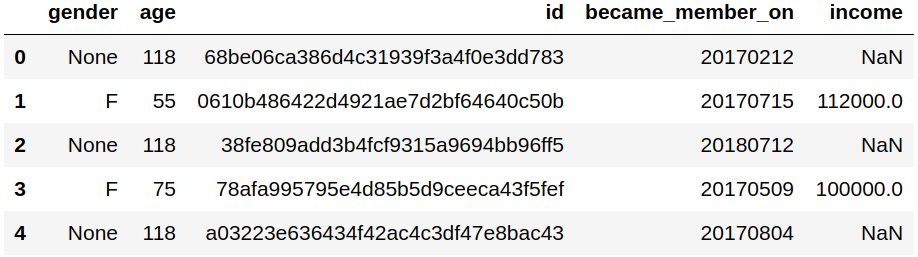
\includegraphics[width=0.8\textwidth]{fig/profile_head.jpg}
	\vspace*{-0.1in}
	\caption{Sample from the portfolio dataset}
	\label{fig1}
	\vspace*{-0.2in}
	\bigskip
\end{figure}

\subsection*{portfolio.json}
The portfolio.json file contains the data of the offers sent during the test period in fields (10 offers): 
\begin{itemize}
	\item reward: (numeric) money awarded for the amount spent
	\item channels: (list) web, email, mobile, social
	\item difficulty: (numeric) money required to be spent to receive reward
	\item duration: (numeric) time for offer to be open, in days
	\item offer\_type: (string) BOGO, discount, informational
	\item id: (string/hash)
\end{itemize}

\begin{figure}[h]
	\centering
	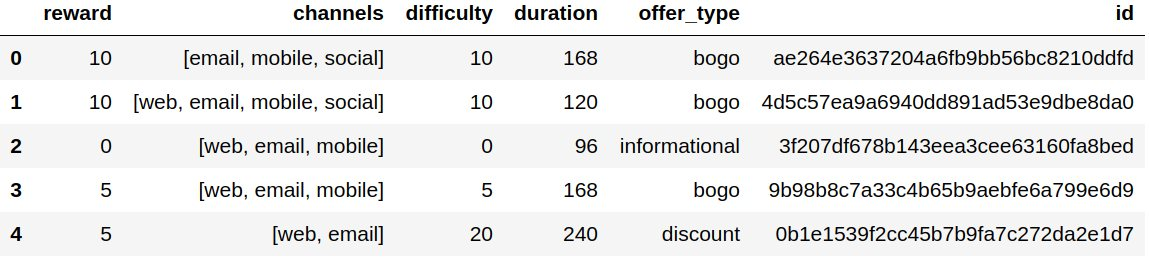
\includegraphics[width=0.7\textwidth]{fig/portfolio_head.jpg}
	\vspace*{-0.1in}
	\caption{Sample from the profile dataset}
	\label{fig2}
	\vspace*{-0.2in}
	\bigskip
\end{figure}

\subsection*{Transcript.json}
The transcript.json file contains timestamped data about transaction and offers in the following fields ((306648 events):
\begin{itemize}
	\item person: (string/hash)
	\item event: (string) offer received, offer viewed, transaction, offer completed
	\item value: (dictionary) different values depending on event type
	\subitem offer id: (string/hash) not associated with any "transaction"
	\subitem amount: (numeric) money spent in "transaction"
	\subitem reward: (numeric) money gained from "offer completed"
	\item time: (numeric) hours after start of test
\end{itemize}

\begin{figure}[h]
	\centering
	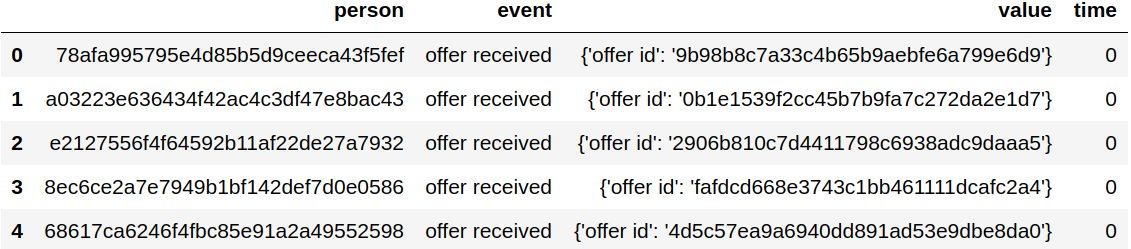
\includegraphics[width=0.9\textwidth]{fig/transcript_head.jpg}
	\vspace*{-0.1in}
	\caption{Sample from the transcript dataset}
	\label{fig3}
	\vspace*{-0.2in}
	\bigskip
\end{figure}

This data in itself is not very informative, so serious effort has to be made to extract meaningful features from it. The feature extraction / engineering is going to be shown in section \ref{sec3}

\subsection{Data Exploration}\label{sec2.2} 

\subsubsection{Dealing with missing values}
As it can be seen in Figure \ref{fig1}, the portfolio dataset is not complete. By examining the data we have established that there are two kinds of data points: One in which all data is provided and one in which gender, age and also income is missing. This can be due to several reasons, one of which is that these people did not agree with the company's privacy policy.

A total number of 2175 datapoints are effected by missing values. One have to deal with these datapoints. A potential solution would be to discard these datapoints from the dataset. However these people possibly form an interesting group in the dataset, so we decided to keep these datapoints as well. These datapoints will be clearly differentiated from the other datapoints by giving them a gender 'U' (unknown). The age and income values will be filled with the respective mean values. The unknown gender category seems to be a reasonable choice for the following reason: Filling up the missing values with the respective means seriously changes data distribution. By the extra gender group we hope to separate these points from all the other ones sufficiently.

\subsubsection{Profile Data Exploration}
There are 8484 Male and 6129 Female datapoints in the dataset. In this respect the number male and female datapoints is quite well balanced, so no care has to be taken on compensating it in any direction. The number of people who classify themselves into other genders is however very small. These people are decided to be kept in the dataset but we assume that the predictions on them will not be very accurate.

The membership length is calculated for the people counting from the date of the last person who got a membership. This is an arbitrary choice, however since we are only interested in the relative lengths of the memberships (the data is going to be normalized / standardized) it works totally fine. After this, the age, income and membership length distribution of the costumers can be analyzed. These distributions, also separated based on genders can be seen in Figure \ref{fig4}.

\begin{figure}[h]
	\centering
	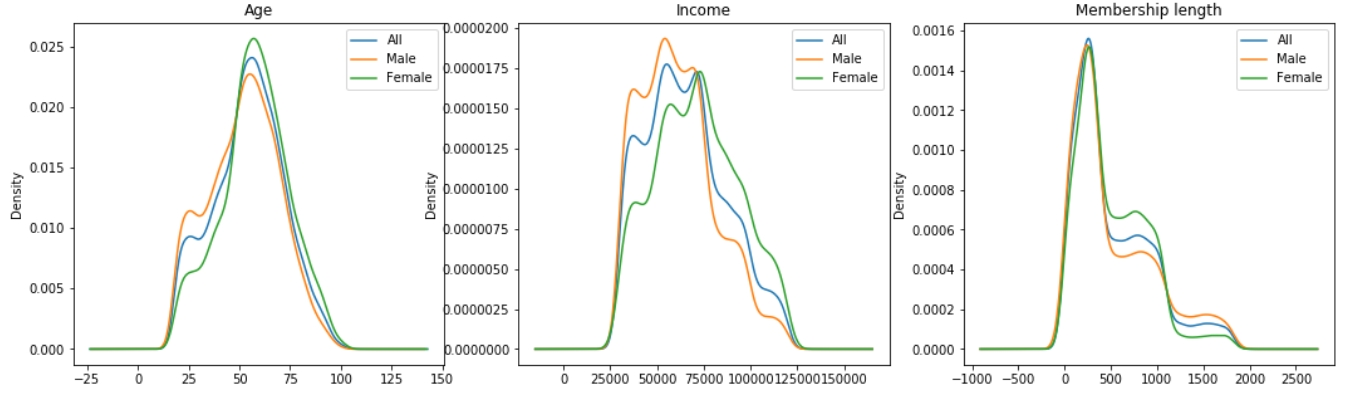
\includegraphics[width=0.99\textwidth]{fig/profile_distributions.jpg}
	\vspace*{-0.1in}
	\caption{Distributions of the age, income and membership data in the dataset}
	\label{fig4}
	\vspace*{-0.2in}
	\bigskip
\end{figure}

From the above plots we derive the following conclusions:
\begin{itemize}
	\item The age distribution is relative nice. It has got a small peak around 25 years, but we assume that it will not pose a serious problem during training.
	\item The income is not perfectly well distributed, it has got some local peaks at certain points. However it will possibly be sufficient for training. There are some differences between the male and female distributions. The male costumers tend to have lower income than the female costumers.
	\item The membership length on the other hand is quite badly distributed. It has a huge peak between 0 and 500. Other than that, there tend to be some intervals where the distribution is almost constant. This left skewed distribution will probably require some transformation before using it for training.
\end{itemize}

Based on these experiments we conclude that it will probably be sufficient to only standardize the age and income distributions and only the membership length data needs to be transformed to behave better during training.

\subsubsection{Offer Data Exploration}

For being able to explore the transcript data, first the field "value" has to be extracted. 3 new columns, called "offer\_id", "amount" and "reward" are created and are filled with the values from the "value" column's dictionaries. 

As it will be seen later, we mostly create our features from statistical data about the offers the costumers receive. For this reason firs we observed some properties of the offers related data in the transcript dataset. We checked the number of received, viewed and completed offers from each type. (From now on we use the phrase "offer" both for actual offers and for simply informational material.) Obviously an informational material can not be completed, however it can be viewed. The distributions can be seen in Figure \ref{fig5}. (The numbers 0-9 correspond to different offers. These were assigned to the offers based on their order in the portfolio dataset)

\begin{figure}[h]
	\centering
	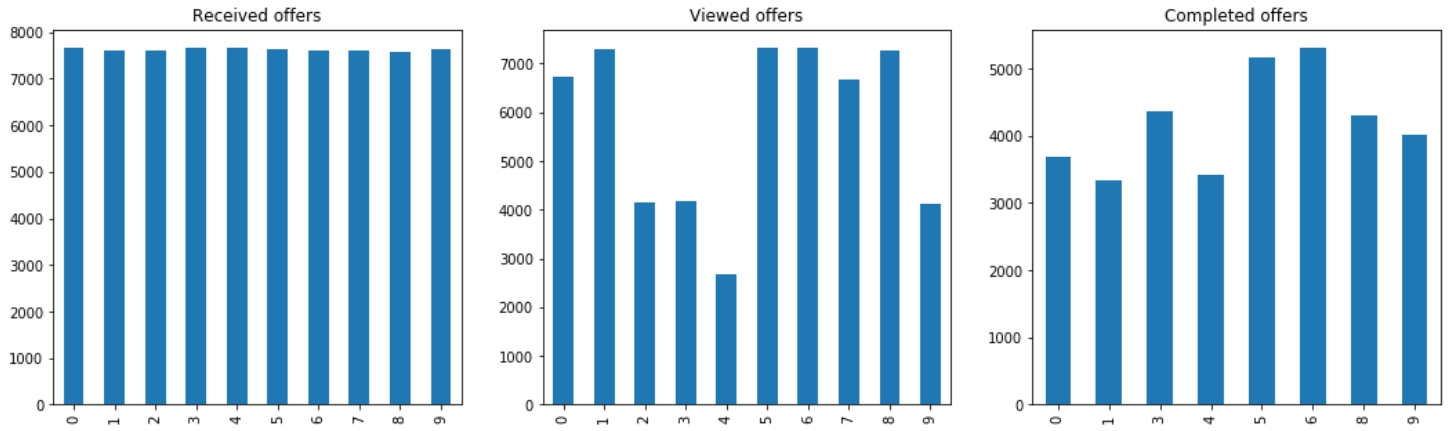
\includegraphics[width=0.99\textwidth]{fig/offer_distributions_1.jpg}
	\vspace*{-0.1in}
	\caption{Number of offers received, viewed and completed}
	\label{fig5}
	\vspace*{-0.2in}
	\bigskip
\end{figure}

The following observations can be made based on these figures:
\begin{itemize}
	\item The amount of sent out promotions is almost the same for every offer type.
	\item The amount of viewed promotions varies stronger and by far the least people viewed the promotion with the highest difficulty and longest duration.
	\item The completion is also relatively homogeneous. (The offer types 2 and 7 correspond to the informational type offers which can not be completed, hence these are missing from the table.)
\end{itemize}

After this we have examined how the distribution of the success of the offers look like. For this we have calculated for every person in the dataset, how many times he/she a) viewed, b) viewed and completed and c) not viewed but still completed an offer. The resultant numbers can be examined in Figure \ref{fig6}. (The x axis of the plots represent the amount of offers per person that fulfills the property indicated in the plot title and the y axis represents the number of people.)

\begin{figure}[h]
	\centering
	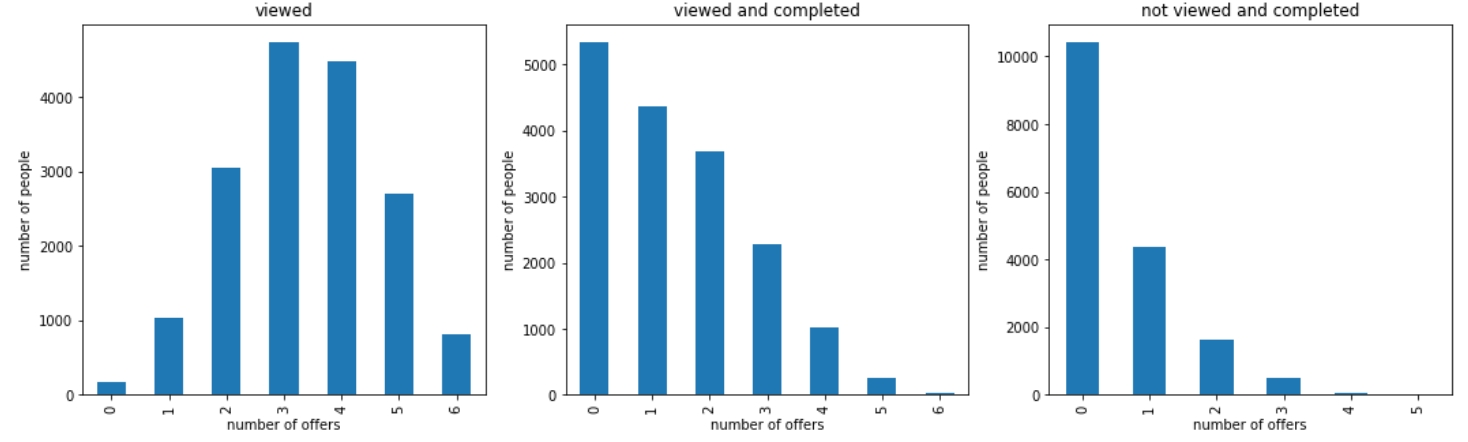
\includegraphics[width=0.99\textwidth]{fig/offer_distributions_2.jpg}
	\vspace*{-0.1in}
	\caption{Sample from the transcript dataset}
	\label{fig6}
	\vspace*{-0.2in}
	\bigskip
\end{figure}

These plots look quite like what we expected:
\begin{itemize}
	\item The number of viewed offers is quite normally distributed. It is not very common that people never look at offers not that they view every single offer they receive.
	\item The number of people who view and then complete an offer several times decreases linearly with the number of occurrences.
	\item  The number of people who view and then complete an offer several times decreases in an exponential-like fashion. It is very improbable, that someone would complete several offers accidentally without knowing about the offer. 
\end{itemize}

\subsubsection{Transaction data Exploration}
A huge part of the transcript dataset are transactions. In the followings we derive some conclusions about these data.

During exploration of the transactions data we have quickly realized that there are some outliers which seriously distort the statistics about the data. The issue can easily be seen in Figure \ref{fig7} where the distribution of the amount of a single transaction is shown:
\begin{figure}[h]
	\centering
	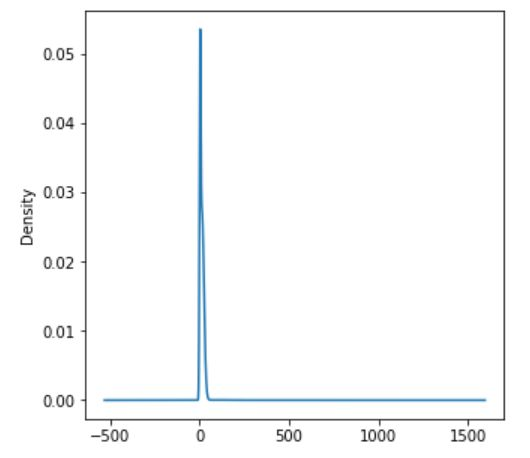
\includegraphics[width=0.4\textwidth]{fig/transaction_distribution_1.jpg}
	\vspace*{-0.1in}
	\caption{Effect of outlier transaction}
	\label{fig7}
	\vspace*{-0.2in}
	\bigskip
\end{figure}

There is an outlier transaction with an amount of 1062.28\$ although the mean for the whole dataset is around 12.7\$. Most of the data is in a normal range, however there are some unlikely high values in the dataset.

A very similar can be said about the cumulative amount of money a person sent during the 30 day period. The mean value for the cumulative spent amount is around 104\$, however the maximum value is 1608\$. Also there are a total number of 422 people who did not spend any money during this period. In Table \ref{table1} we show the number of people who spent more than a specified threshold.

\begin{table}[h] \label{table1}
	\begin{center}
	\begin{tabular}{ c | c | c | c | c | c | }
		& $>100$ & $>200$ & $>300$ & $>500$ & $>1000$\\
		\hline
		number of people & 6722 & 2349 & 738 & 272 & 48 \\
		\hline  
	\end{tabular}
	\end{center}
	\caption{Number of people in the dataset who spent more than different thresholds during the 30 days.}
\end{table}

We decided that some people should be excluded from the data for the following two reasons:
Either they are not representative for the whole group, or they are not the target who the company should consider when they plan their advertisement campaign. By not being representative we mean, that a portion of the group spends much more money than the rest of the group. They are outliers in the dataset and would just reduce the performance of the model. The second group is the people who have not spent any money during the 30 day period. These people should not be considered as potential costumers and hence can be discarded from the dataset. 

In Figure \ref{fig8} the distribution of the cumulative amount spent by a person can be seen if a group of people whose purchases are over a specified threshold are discarded from the data.

\begin{figure}[h]
	\centering
	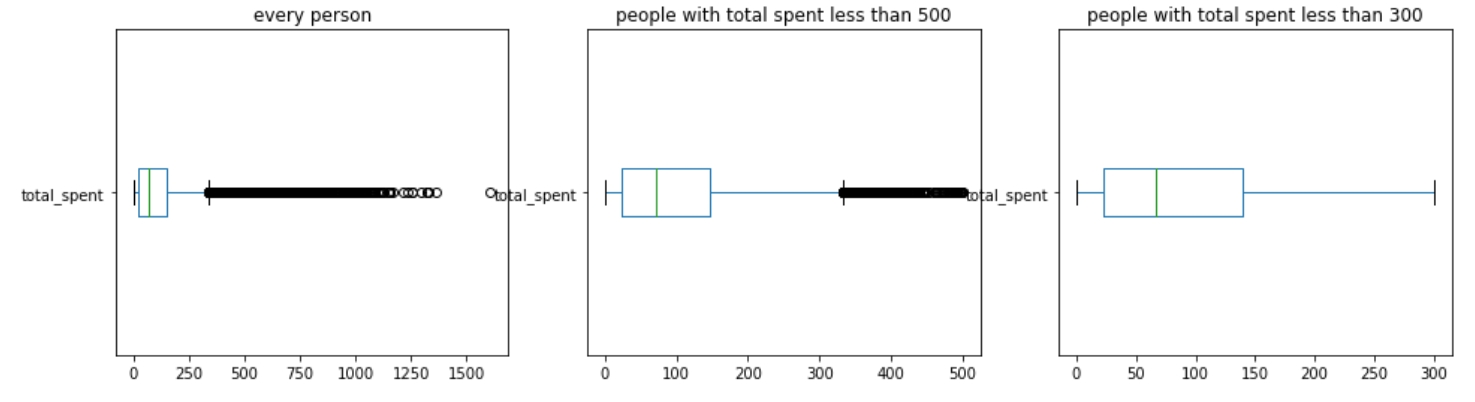
\includegraphics[width=0.99\textwidth]{fig/transaction_distribution_2.jpg}
	\vspace*{-0.1in}
	\caption{Distribution of cumulative money spent during the 30 day period}
	\label{fig8}
	\vspace*{-0.2in}
	\bigskip
\end{figure}

On the first two figures one can see the effect of outlier data in the dataset. Based on these experiments we have decided to discard the people (and all data related to them) from the dataset, who either have spent 0\$ or more than 300\$ during the 30 day period. This means that a total number of 1160 people will be dropped from the data. This is only 6.8\% of the people and we assume that around the same amount of data will be lost from the transcript dataset.

\subsection{Algorithms and Techniques}\label{sec2.3}

It is a crucial step to preprocess the data that later will be fed to the model during training. To be able to decide which preprocessing steps are required for which features data visualization is unavoidable. After we have obtained some characteristics of the data through visualization we concluded that the following algorithms are going to be use through preprocessing:

The age and income features are relatively nicely distributed and hence will only have to be standardized. We would like to carry out the standardization before filling up the missing values with the respective means, since otherwise these would distort the data strongly. We have chosen sklearn's StandarScaler algorithm since it is able not to consider "None" type values. The scaler standardizes the data using the following formula:
$$x_{scaled} = \frac{x - \mu}{\sigma}$$
where $\mu$ is the mean and $\sigma$ is the standard deviation of the feature calculated for the whole dataset.

The membership length is a strongly left skewed distribution and hence has to be transformed. For this we have chosen to use sklearn's QuantileTransform algorithm. This method transforms the features to follow a uniform or a normal distribution using quantiles information. Therefore, for a given feature, this transformation tends to spread out the most frequent values.

Due to the reasons detailed in the previous subsections, the people and all data related to them, who tend to be outliers because of their spending are going to be removed from the dataset.

An important part of the solution that we have chosen is the generation of training data from the provided dataset. This algorithm is going to be detailed later in the Methodology section.

\subsubsection{Chosen model}

we are going to train a feed forward neural network to predict into which category an offer is going to fall after it is sent to a costumer. Feed forward neural networks are relatively easy to train and are universal approximators in the sense, that an infinitely complex neural network can approximate any given nonlinear function. This does not necessarily mean that neural networks are the best choice for every task. However they are quite usual choices for data where one suspects very tricky underlying distribution as it is in this case. 

The neural network is going to be implemented using the PyTorch framework.

\subsection{Banchmark Model}\label{sec2.4}

We have chosen an easily implementable and easy to evaluate model as benchmark model. A kNN (k Nearest Neighbor) model is going to be used. As we suspect that similar people react similarly to offers a kNN classifier will possibly perform quite well for the task and hence will be a good benchmark model to compare the performance of the neural network to.




	\section{Methodology} \label{sec3}

In the previous section some issues were identified with the dataset. The \textit{Algorithms and Techniques} subsection details the algorithms that were used to remedy these issues. In this section we show the results that were acquired during data preprocessing.

The other important contribution of this section is the feature engineering part. This provides details about how the features from the dataset were extracted.

\subsection{Preprocessing the Portfolio Dataset}

We do not use much data about the portfolio dataset. We do realize that some interesting features could have also been extracted from this data, however we decided to focus on other features of the data. In the full created feature vectors the offer that was received is one-hot-encoded to be able to feed it to the neural network. Also the duration of the offers is converted to hours to be able to use it with the transcript dataset where the timestamp is provided in hours instead of days.

\subsection{Preprocessing the Profile Dataset}

Due to the reasons detailed in the previous section we removed the people who have spent more than a total of 300\$ or did not spend anything. With this we have removed 6.8\% of the profile and and 7.3\% of the transcript data. These are not very large percentages, so there are plenty of data remaining after this selection.

After this, we have one-hot-encoded the gender into the following categories: "F", "M", "O" and "U". 

Before filling up the "None" type values in the dataset, the age and income fields are standardized using sklearn's StandardScaler algorithm. The features before and after standardization can be seen on Figure \ref{fig9}

\begin{figure}[h]
	\centering
	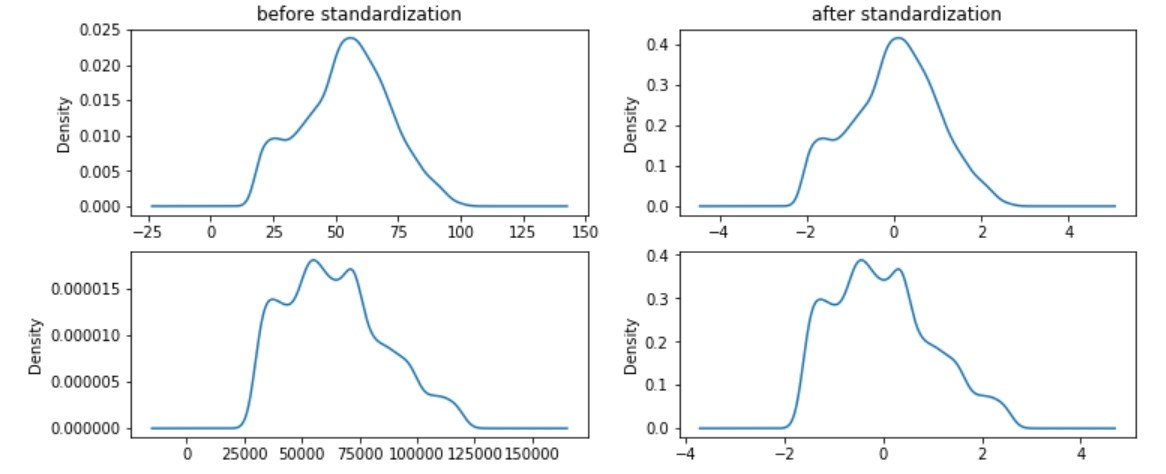
\includegraphics[width=0.8\textwidth]{fig/age_before_after.jpg}
	\vspace*{-0.1in}
	\caption{Age and income before and after standardization}
	\label{fig9}
	\vspace*{-0.2in}
	\bigskip
\end{figure}

After standardizing the age and income data, the missing values can be filled with the respective means. 

Next the membership length is calculated and since it was shown that it has a quite distorted distribution, it will be transformed using sklenarn's QuintileTransform algorithm. After that the resultant data is also standardized. The data before and after the transformation can be examined in Figure \ref{fig10}.

\begin{figure}[h]
	\centering
	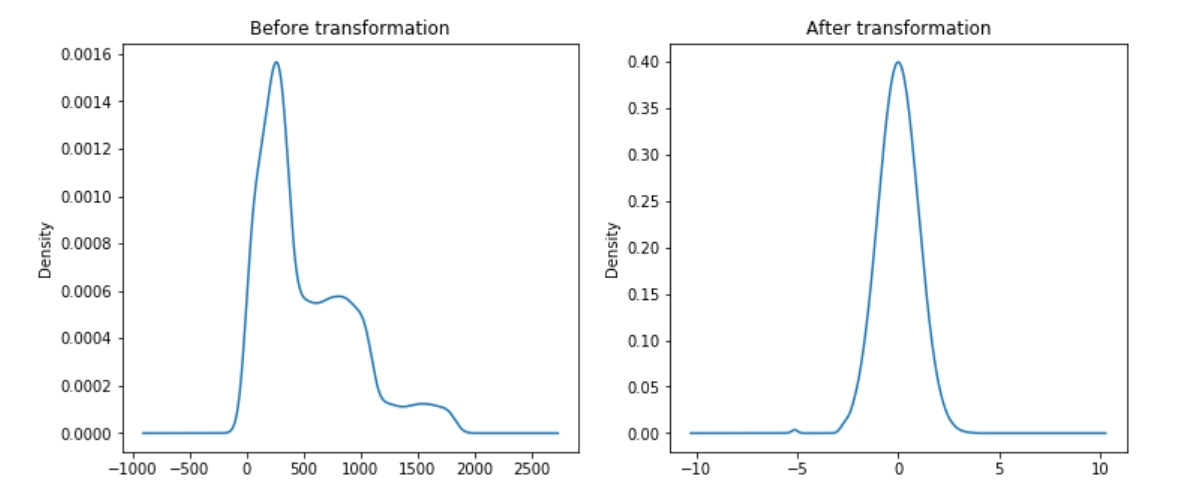
\includegraphics[width=0.8\textwidth]{fig/membership_before_after.jpg}
	\vspace*{-0.1in}
	\caption{Membership length before and after the transformation and standardization.}
	\label{fig10}
	\vspace*{-0.2in}
	\bigskip
\end{figure}

After the data was preprocessed and cleaned it is ready for handcrafted feature creation.

\section{Handcrafted Features}



	\section{Results} \label{sec4}

After carrying out carefully the data preprocessing, feature engineering and training steps, we have obtained the trained classifier. In this section we are going to present the results of the training. 

\subsection{Model Evaluation and Validation}

After validating by overfitting to a single training example that the model is implemented correctly and is able to learn we carried out a hyperparameter search in the parameter space. The hyperparameters were chosen with which the highest validation accuracy was acquired. These parameters are provided in section \ref{sec3.4}. The model was then fully trained with these parameters. The training and validation loss during training can be examined in Figure \ref{fig12}

\begin{figure}[h]
	\centering
	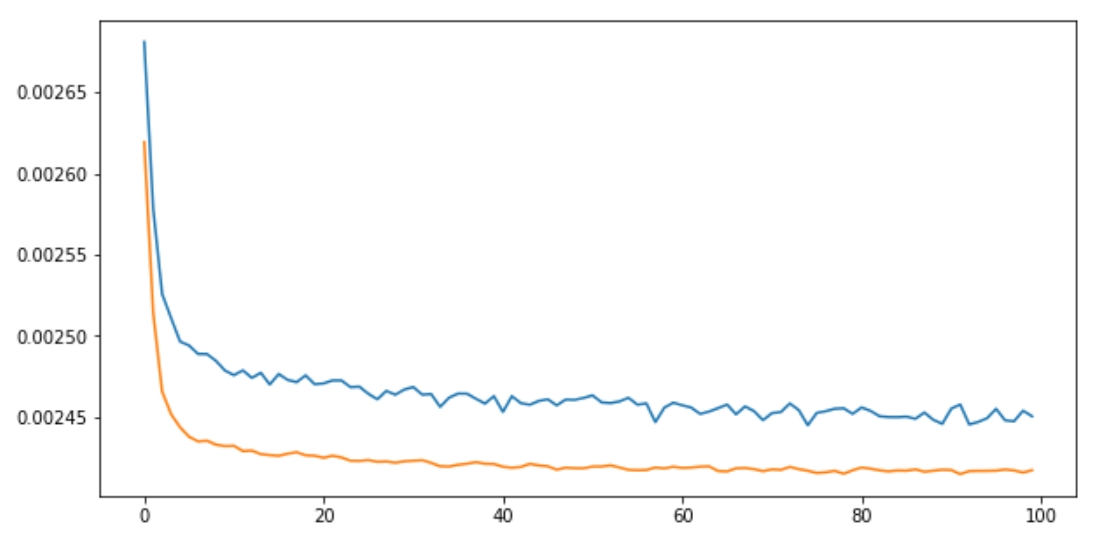
\includegraphics[width=0.7\textwidth]{fig/loss.jpg}
	\vspace*{-0.1in}
	\caption{Training (blue) and validation (orange) loss during training.}
	\label{fig12}
	\vspace*{-0.2in}
	\bigskip
\end{figure}

From this figure one can conclude that the training has converged to a local optima. The regularization is also sufficient as the model does not overfit to the data. (Does not memorizes the labels of the training set.) The phenomena that the validation loss is smaller than the training loss is thanks to the regularization technique. Since dropout is only used during training and is switched off during validation, the validation loss becomes lower during training. 

After training, the model was evaluated on the test set which was never shown to the model before. On the test set the model was able to reach an accuracy of 52\%. 

The benchmark model was also evaluated with different number of neighbors. It was able to produce an accuracy of 46\% with k=10 neighbors. 

Hence we conclude that the trained neural network was able to outperform the kNN classifier slightly. Further analysis and justification of the results is provided in the next subsection.


\subsection{Justification}

The successfully trained model was tested on the test set which was never seen before. It acquired 52\% accuracy on this set. This is a slight improvement compared to the accuracy of the benchmark kNN classifier (46\%). 

Although this accuracy does not seem to be very high, let us place it into context. We have also expected a somewhat higher accuracy than this number. 52\% accuracy means that only in slightly more than half of the cases the future of a received offer were predicted successfully. In other words, the classifier is only able to predict the reaction of every second costumer. 

However one have to consider the following properties of the situation to be able to evaluate the performance in its context. First of all, the received offers are classified into 4 classes. This means that a random classifier would achieve an accuracy around 25\%. Our classifier has reached an accuracy more than twice as high. Also a very important aspect that one has to keep in mind is how dynamically change the behavior of the people. It really is a stochastic environment. It is totally possible, that someone have completed a certain offer 5 out of 5 times before and still does not completes it the $6^{th}$ time. People behave so stochastically that it is impossible to tell their reaction to certain offers with a very high accuracy. 

In this respect we conclude that although this accuracy is not very high, it is still a surprisingly good result considering the complexity and randomness of the task it solves. Being able to predict the exact outcome of an advertising campaign for every second person could be a very powerful tool for companies such as Starbucks.

\subsection{Summary}

In this report we have detailed our solution for Starbuck's Capstone Challenge. Our chosen aim was to try to predict, into which of the following four classes a received offer is going to fall given some basic data about the person who receives the offer and its costumer history until receiving the offer.:

\begin{itemize}
	\item Will not be viewed nor completed accidentally
	\item Will not be viewed but will be completed
	\item Will be viewed but will not be completed
	\item Will be completed and viewed
\end{itemize}

We have explored the provided data thoroughly, identified the issues with it and provided solutions to remedy them. We have preprocessed the dataset to make it sufficiently well behaving for training and developed a feature representation which from our point of view describes the costumers and their costumer history until receiving the offer accurately. We have extracted the features from the raw dataset and created the corresponding labels.

We have implemented a feed forward neural network for the above classification purpose. After searching the sufficient hyperparameters, we have trained the network with the training data. We then compared its results with our benchmark model, which is a kNN classifier with 10 neighbors.

We have reached an accuracy of 52\% on the testing set, which is a slight improvement on the kNN classifier which have reached 46\%. Although these accuracy numbers do not seem to be very high, considering the randomness on how people act in the real word, these numbers are quite impressive in our point of view. For every second person one is able to predict exactly what the future of an offer is going to be. 

This can be a powerful tool for companies. Considering the accuracy of the model, a useful application of such a model would be to check the success of a campaign for a large number of costumers and obtain whether for most of the people it would be successful or not. 


\subsection{Outlook}

After training the model, we have also trained an other network for a slightly different purpose. We have re-classified the received offers only into successful and not successful categories. We considered the offers to be successful if they were viewed and completed or if they were plain informational offers and they were viewed. We have trained a neural network with the same features for this binary classification task. 

We were able to obtain the following results with it:
\begin{itemize}
	\item accuracy: 65\%
	\item precision: 49\%
	\item recall: 75\%
	\item false negative rate: 25\%
\end{itemize}

From these measures the high recall and low false negative rate are especially appealing. This means that the model mostly classifies successful outcomes correctly and most of the failures are made by classifying some offers to be successful although they will not be successful in fact. This is the smaller problem. A bigger problem would be if customers who would otherwise not receive the offer do not receive the offer at all.

In this respect a further improvement in this direction could be an interesting field of further research.















	
	
	
\end{document}